\frame{
  \frametitle{Trees!}
  \begin{columns}
      \begin{column}{0.4\textwidth}
         \begin{itemize}
            \item Trees are the building block of most data structures.
        
            \medskip
            
            \item Every node has one parent, except for the root which has no parent.
        
            \medskip
        
            \item Nodes with no children are leaves, nodes with children are internal nodes.
          \end{itemize}
      \end{column}
        \begin{column}{0.6\textwidth}
            \begin{center}
            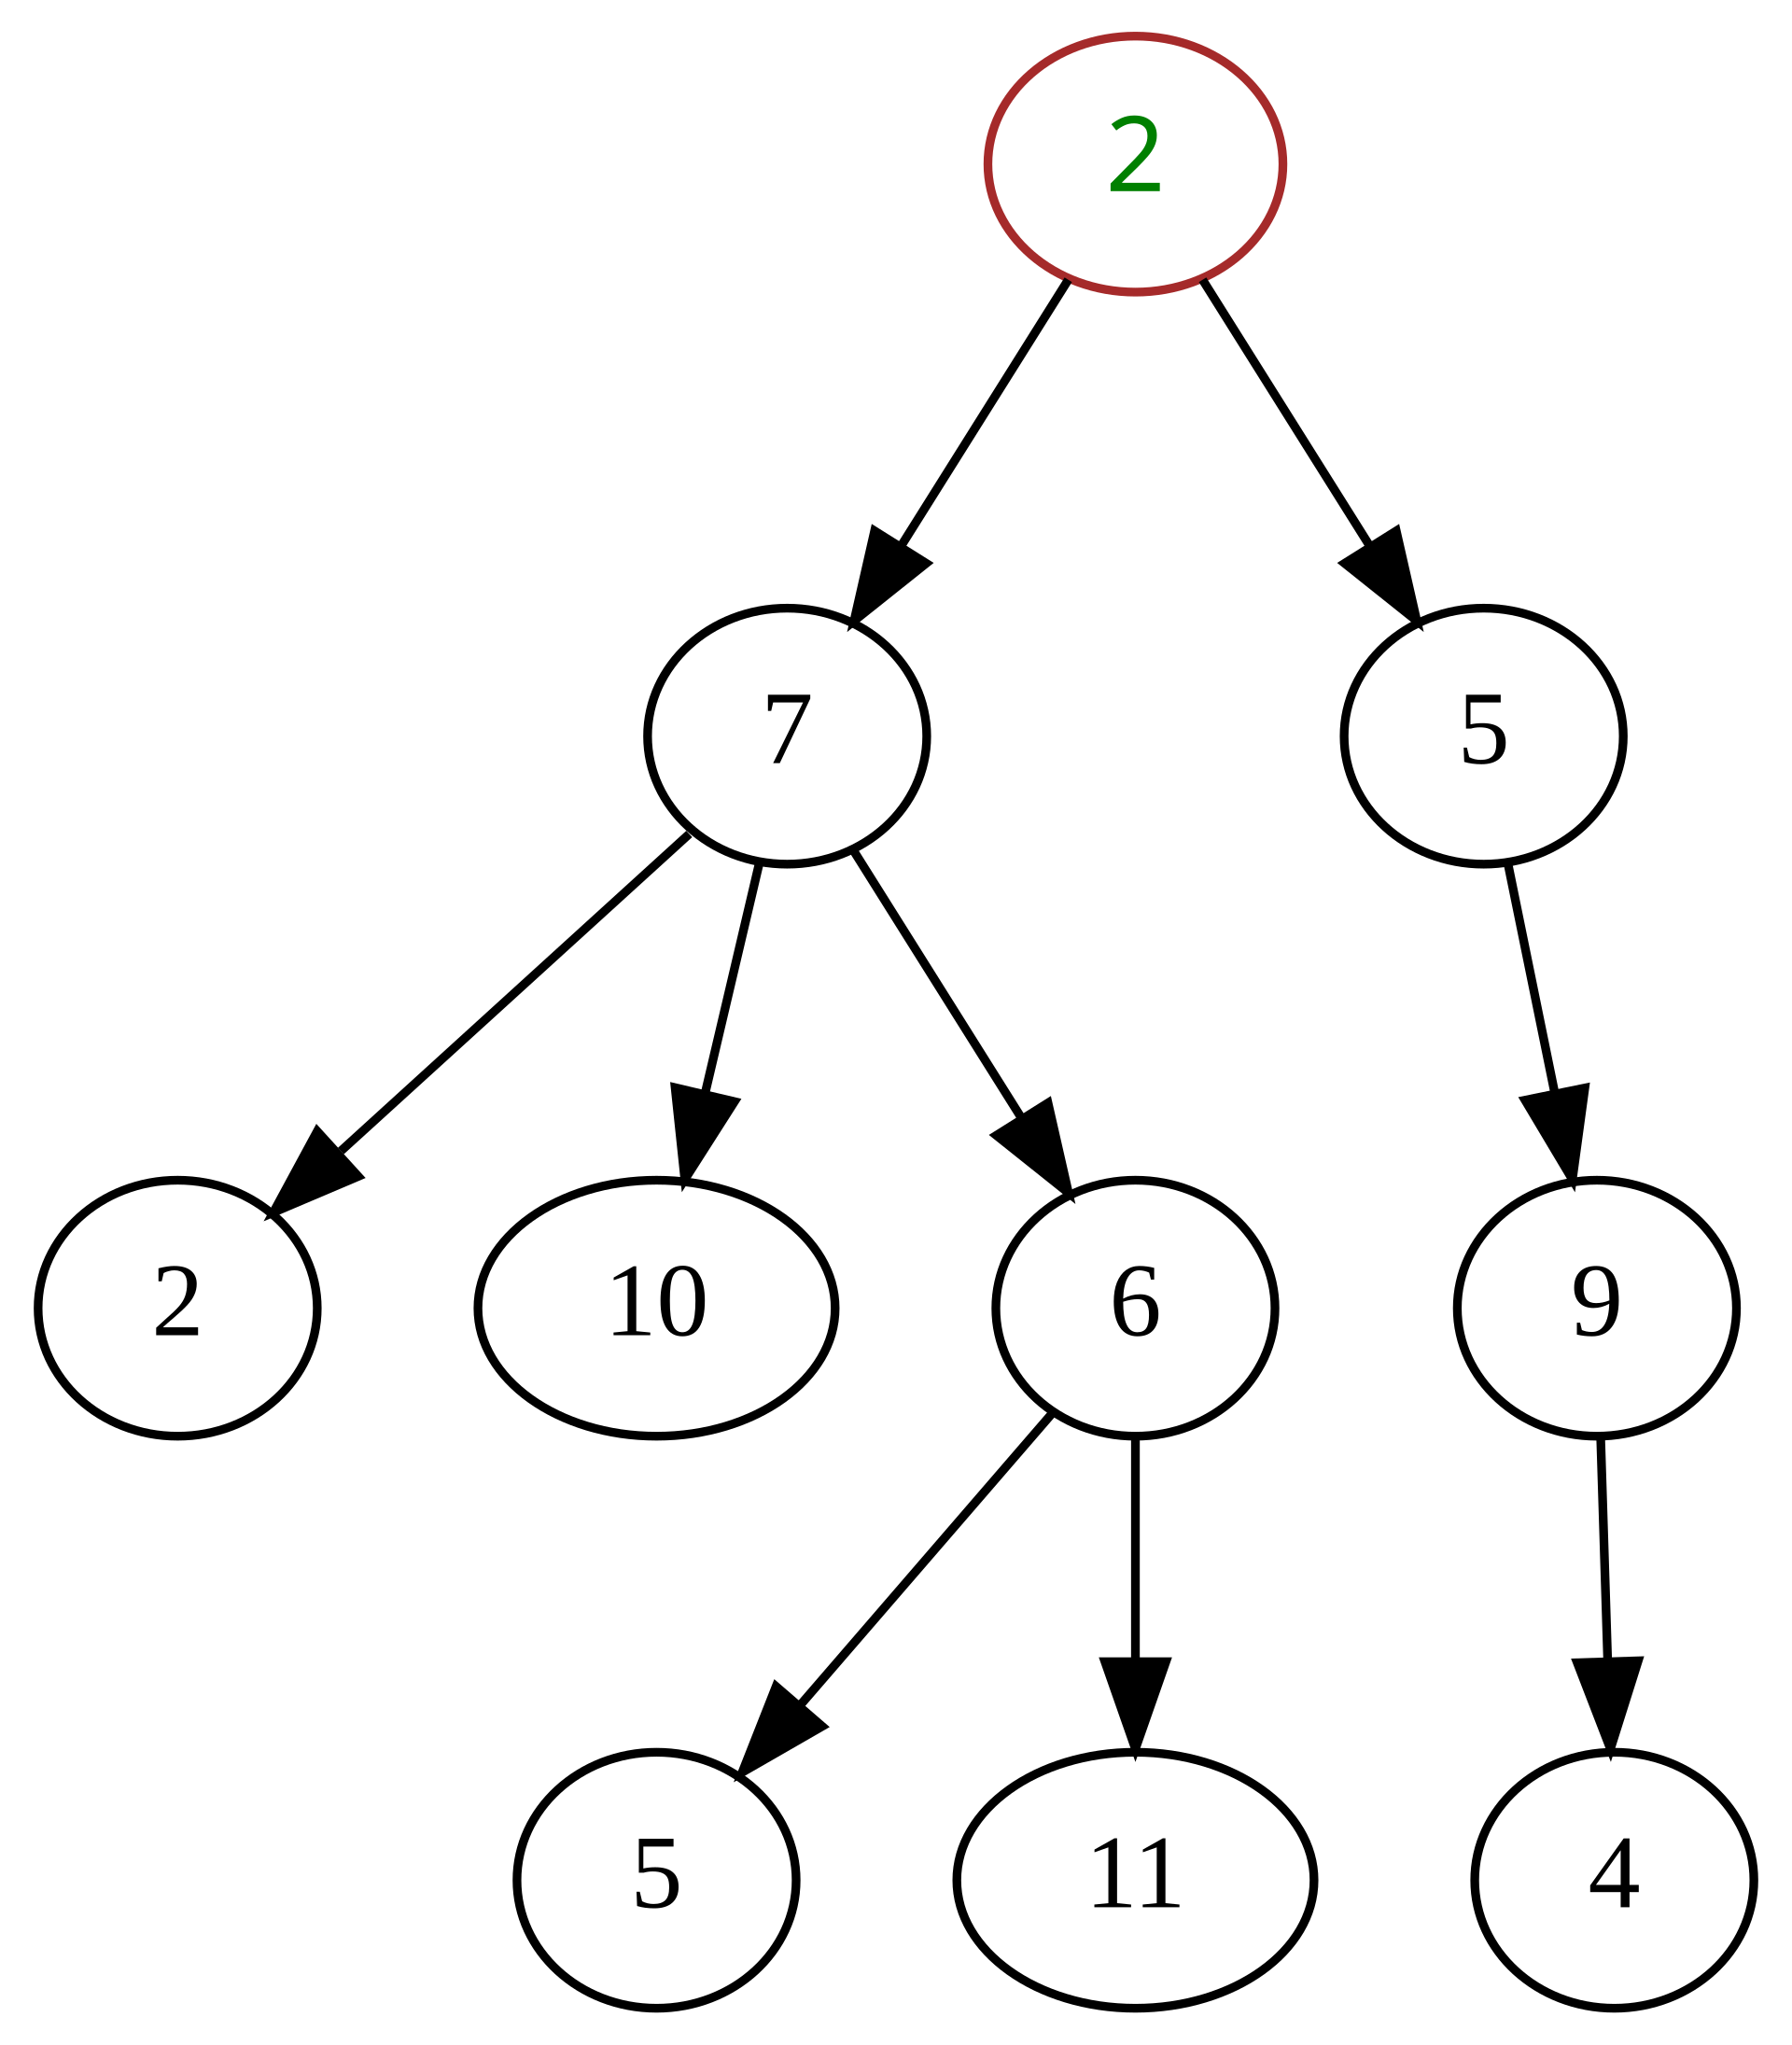
\includegraphics[scale=0.07]{slides/alphabet_trees/Tree_(computer_science).svg.png}

            {\tiny \texttt{By Paddy3118 - Own work, CC BY-SA 4.0, https://commons.wikimedia.org/w/index.php?curid=83223854}}
            \end{center}
        \end{column}
  \end{columns}
}




\frame{
  \frametitle{A-Z of Trees (non-exhaustive)}
  {
  \small
  \begin{columns}
  \def\item{\par\vspace{1ex}}
      \begin{column}{0.25\textwidth}
        \item AVL Trees
        \item B Trees
        \item Cartesian Trees
        \item Decision Tree
        \item Exponential Trees
        \item Fenwick Trees
        \item Gomory-Hu Tree
        \item H-Tree
        \item Interval Tree
        \item Judy Array
      \end{column}
      \begin{column}{0.25\textwidth}
        \item $k$-d Tree
        \item Link-Cut Tree
        \item Merkle Trees
        \item N Tree
        \item Order Statistics Tree
        \item PQ Tree
        \item Quadtree
        \item Red Black Trees
        \item Splay Trees
        \item Tango Trees
      \end{column}
       \begin{column}{0.25\textwidth}
        \item Universal B Trees
        \item Vantage Point Tree
        \item Wallace Tree
        \item X-fast Trie
        \item Y-fast Trie
        \item Zip Trees
      \end{column}
  \end{columns}
  }
}


\frame{
  \frametitle{\sout{Subsections} Subtrees}
 \begin{itemize}
    \item ARSTZ : Balanced Binary Search Trees (BST)

    \medskip
    
    \item BCMUXY : Other Binary Trees

    \medskip

    \item IKQV : Spatial Data Structures

    \medskip 

    \item EFGJLP : Niche data structures

    \medskip 

    \item DHNOW :  Non-data structures
  \end{itemize}
}

\frame{
  \frametitle{\sout{Subsections} Subtrees}
 \begin{itemize}
    \item \textbf{ARS}TZ : Balanced Binary Search Trees (BST)

    \medskip
    
    \item BCMUXY : Other Binary Trees

    \medskip

    \item IKQV : Spatial Data Structures

    \medskip 

    \item EFGJ\textbf{L}P : Niche data structures

    \medskip 

    \item \textbf{D}H\textbf{N}OW :  Non-data structures
  \end{itemize}
}


% \frame{
%   \frametitle{A-Z of Trees}
%   {
%   \small
%   \begin{columns}
%       \begin{column}{0.15\textwidth}
%           \begin{itemize}
%             \item AVL Trees
        
%             \item Red Black Trees
        
%             \item Splay Trees
        
%             \item Tango Trees
        
%             \item Zip Trees
%           \end{itemize}
%       \end{column}
%       \begin{column}{0.15\textwidth}
%            \begin{itemize}
%     \item B Trees

%     \item Cartesian Trees

%     \item Merkle Trees

%     \item Universal B Trees

%     \item X-fast Trie

%     \item Y-fast Trie
%   \end{itemize}
%       \end{column}
%       \begin{column}{0.17\textwidth}
%  \begin{itemize}
%     \item Interval Tree

%     \item $k$-d Tree

%     \item Quadtree

%     \item Vantage Point Tree
%   \end{itemize}
%       \end{column}
%         \begin{column}{0.17\textwidth}
%  \begin{itemize}
%     \item Exponential Trees

%     \item Fenwick Trees

%     \item Gomory-Hu Tree

%     \item Judy Array

%     \item Link-Cut Tree

%     \item PQ Tree
%   \end{itemize}
%       \end{column}
%       \begin{column}{0.17\textwidth}
%  \begin{itemize}
%     \item Decision Tree

%     \item H-Tree

%     \item N??

%     \item Order Statistics Tree

%     \item Wallace Tree
%   \end{itemize}
%       \end{column}
      

%   \end{columns}
%   }
% }